% SECCIÓN PROPIA DE BRENDA. Para integrarla al equipo no modificar main.tex.
\begin{frame}{Brenda | Frontend de usuarios y roles}
  \begin{columns}[T,onlytextwidth]
  \column{0.55\textwidth}
  {\large\bfseries Responsabilidad}\par\vspace{0.14cm}
  \azul{HU-01} Registro y edición de usuarios.\\[0.20cm]
  \azul{HU-02} Asignación de roles y edición de permisos.\\[0.40cm]
  \begin{itemize}\setlength\itemsep{0.18cm}
    \item Separación de preparación de datos y guardado.
    \item Reducción de lógica repetida y dependencia HTTP en formularios.
    \item Revisión de comportamiento mediante compilación y pruebas funcionales.
  \end{itemize}
  \column{0.41\textwidth}
  \cajaclara{\textbf{Evidencia versionada}\\[0.20cm]
  \texttt{eb00464} \; Versión inicial\\[0.12cm]
  \texttt{4cab7eb} \; Refactor HU-01\\[0.12cm]
  \texttt{6ccf4ca} \; Refactor HU-02}
  \vspace{0.24cm}
  {\footnotesize Ruta del código: \texttt{src/Users.tsx}}
  \end{columns}
\end{frame}

\begin{frame}{HU-01 | Registro de usuarios: antes y después}
  \vspace{0.12cm}
  \begin{columns}[T,onlytextwidth]
  \column{0.493\textwidth}
  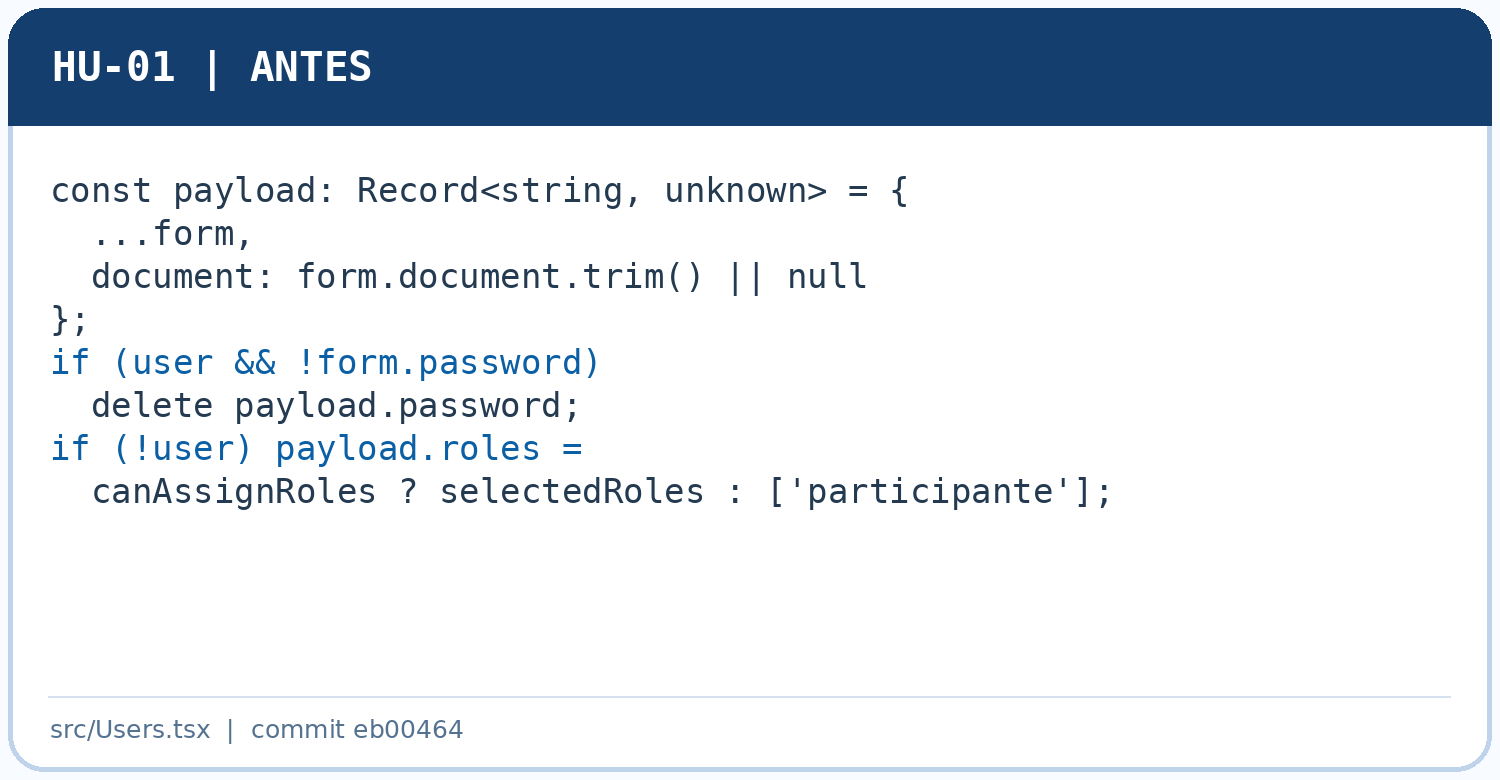
\includegraphics[width=0.90\linewidth]{imagenes/HU01_antes.png}
  \column{0.493\textwidth}
  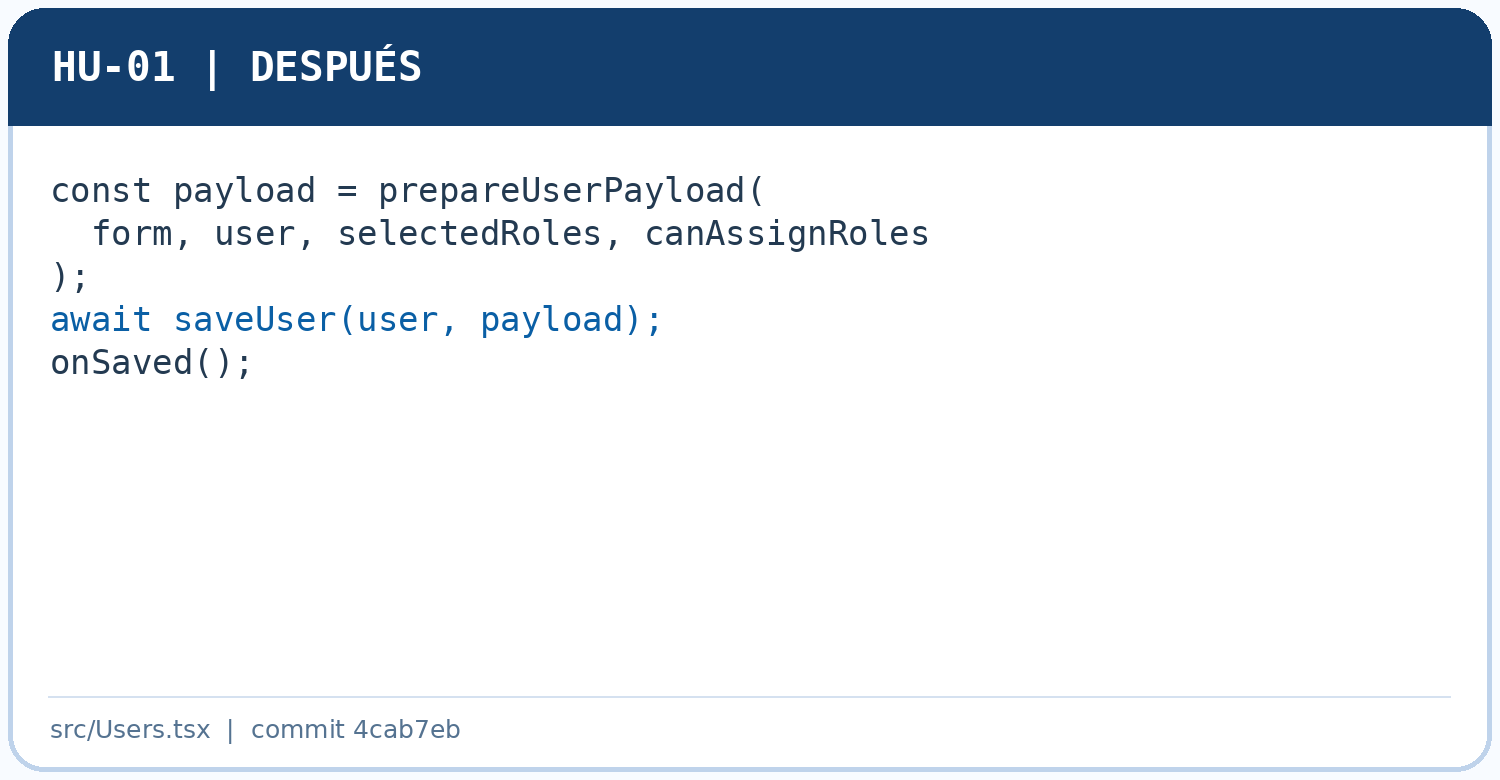
\includegraphics[width=0.90\linewidth]{imagenes/HU01_despues.png}
  \end{columns}
  \vspace{0.03cm}
  \cajaclara{\footnotesize \textbf{Qué cambió:} la preparación del \texttt{payload} y la petición HTTP se extrajeron de \texttt{submit()} a funciones específicas.\\
  \textbf{Por qué:} responsabilidad única, cohesión y menor acoplamiento.}
  \vspace{0.12cm}
  {\tiny Los extractos conservan la lógica del repositorio; saltos de línea adaptados para legibilidad. Fuente: commits \texttt{eb00464} y \texttt{4cab7eb}.}
\end{frame}

\begin{frame}{HU-02 | Roles y permisos: antes y después}
  \vspace{0.12cm}
  \begin{columns}[T,onlytextwidth]
  \column{0.493\textwidth}
  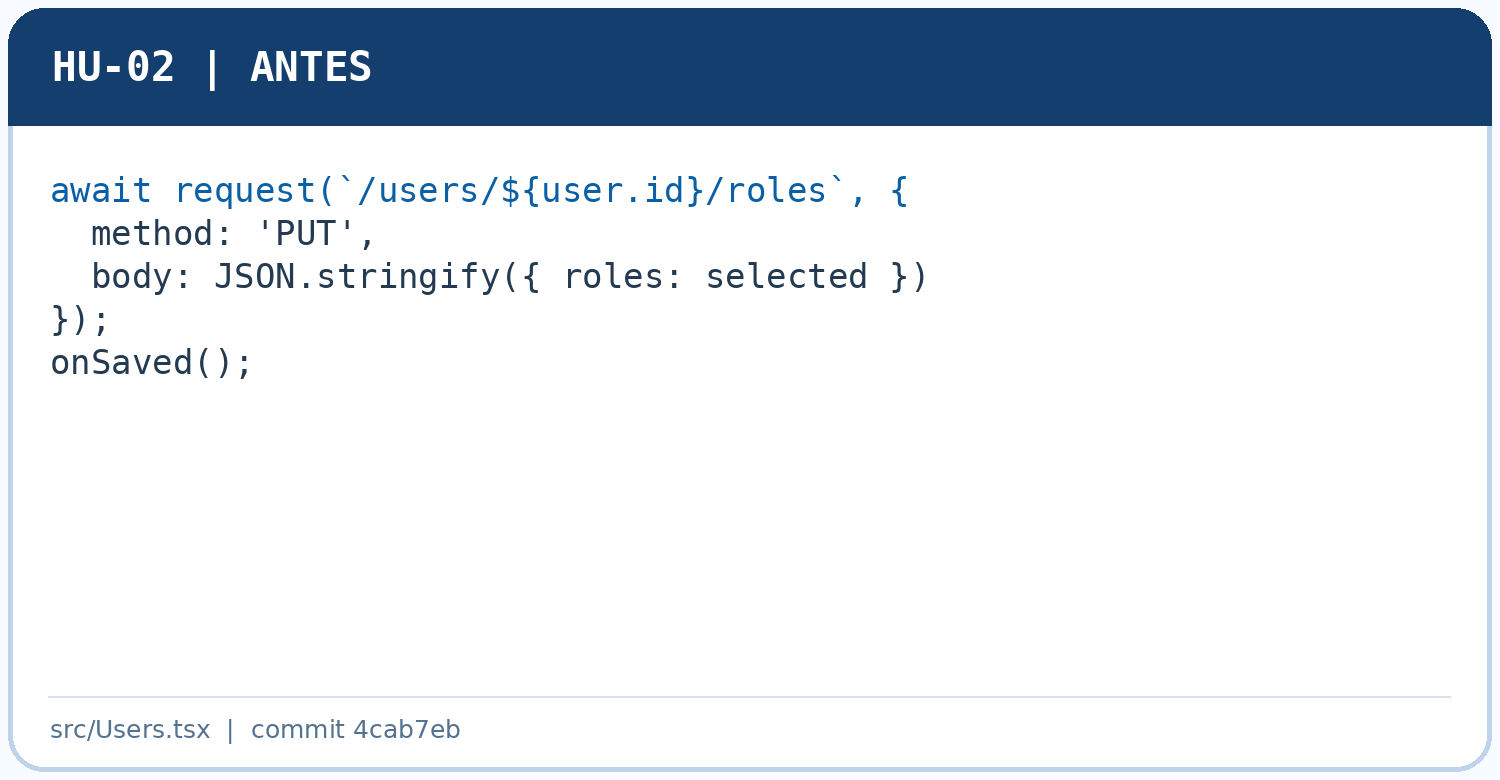
\includegraphics[width=0.90\linewidth]{imagenes/HU02_antes.png}
  \column{0.493\textwidth}
  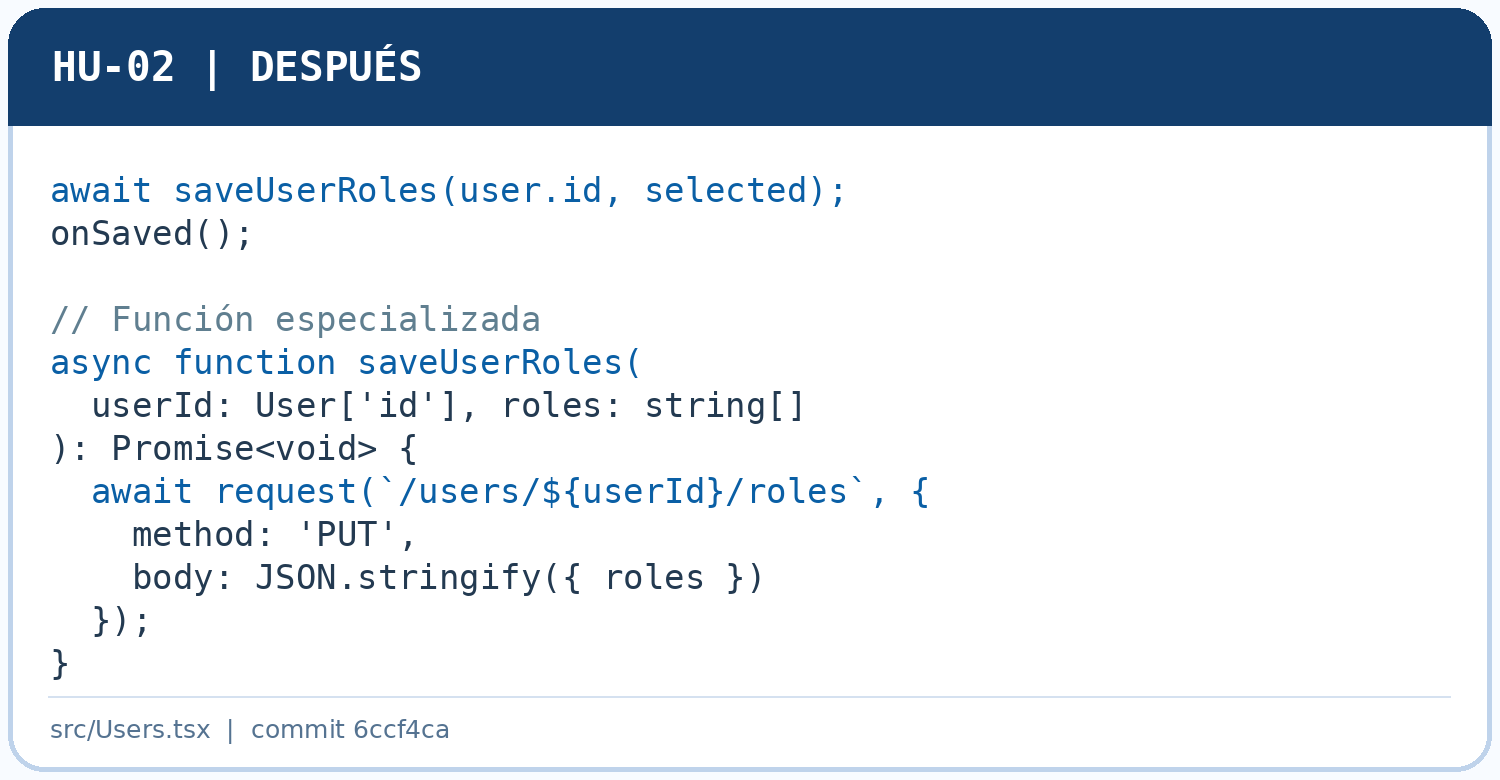
\includegraphics[width=0.90\linewidth]{imagenes/HU02_despues.png}
  \end{columns}
  \vspace{0.03cm}
  \cajaclara{\footnotesize \textbf{Qué cambió:} \texttt{UserRolesForm} usa \texttt{saveUserRoles()}; también se separaron \texttt{saveRolePermissions()}, \texttt{toggleSelection()} y \texttt{loadRoleCatalog()}.\\
  \textbf{Por qué:} reutilización, menor duplicación y separación entre vista y acceso a datos.}
  \vspace{0.12cm}
  {\tiny Extractos basados en los commits \texttt{4cab7eb} y \texttt{6ccf4ca}; líneas ajustadas para la diapositiva.}
\end{frame}

\begin{frame}{Brenda | Verificación y trazabilidad}
  \begin{columns}[T,onlytextwidth]
  \column{0.46\textwidth}
  \begin{block}{Pruebas automáticas del proyecto}
    \vspace{0.18cm}
    {\centering\Huge\bfseries 28\par}
    {\centering\small pruebas aprobadas\par}
    \vspace{0.12cm}
    {\centering\Large\bfseries 0 fallidas\par}
    \vspace{0.14cm}
    {\centering\scriptsize \texttt{npm run check} | TypeScript + Vite OK\par}
  \end{block}
  \column{0.51\textwidth}
  \textbf{Comprobaciones manuales}\par\vspace{0.15cm}
  \begin{itemize}\setlength\itemsep{0.19cm}
    \item Registro de un usuario de prueba.
    \item Asignación de múltiples roles.
    \item Edición de permisos de un rol.
  \end{itemize}
  \vspace{0.20cm}
  \cajaclara{\footnotesize Las \textbf{28 pruebas} son de todo el sistema, principalmente backend. No se presentan como 28 pruebas exclusivas del frontend.}
  \end{columns}
\end{frame}
